\begin{comment}


\begin{center}
\thispagestyle{empty}
%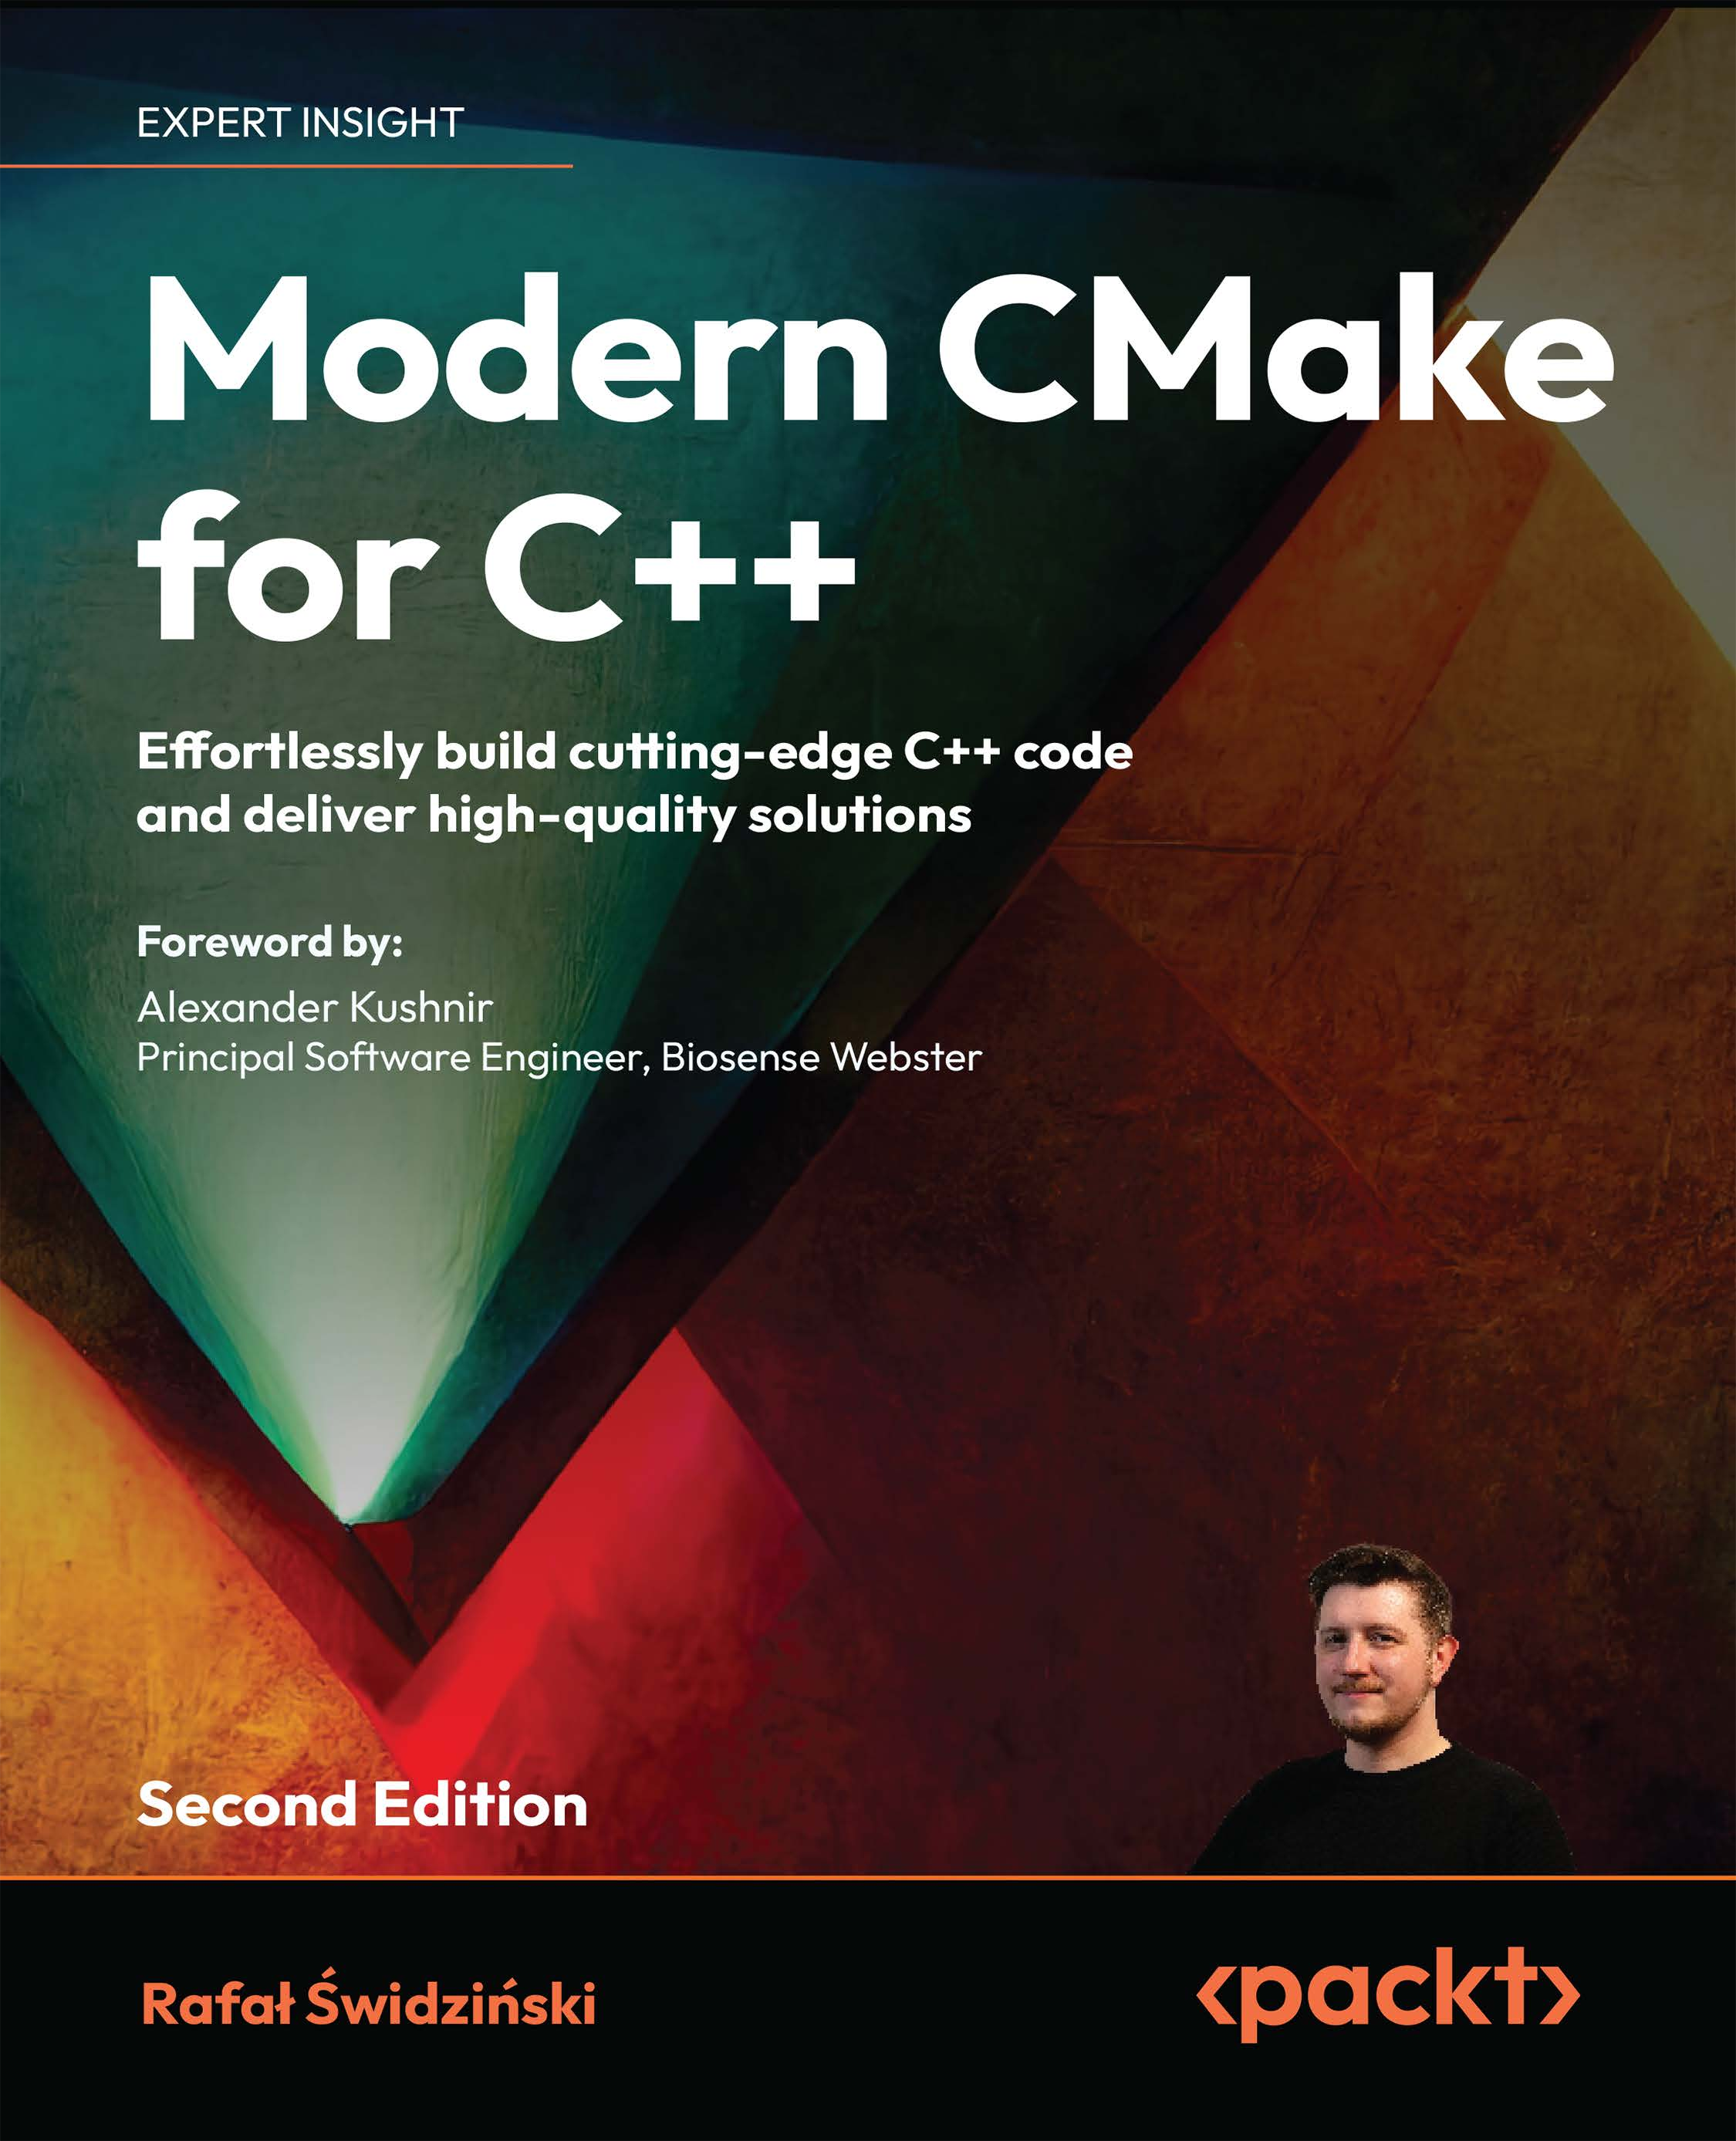
\includegraphics[width=\textwidth,height=\textheight,keepaspectratio]{cover.png}
\begin{tikzpicture}[remember picture, overlay, inner sep=0pt]
\node at (current page.center)
{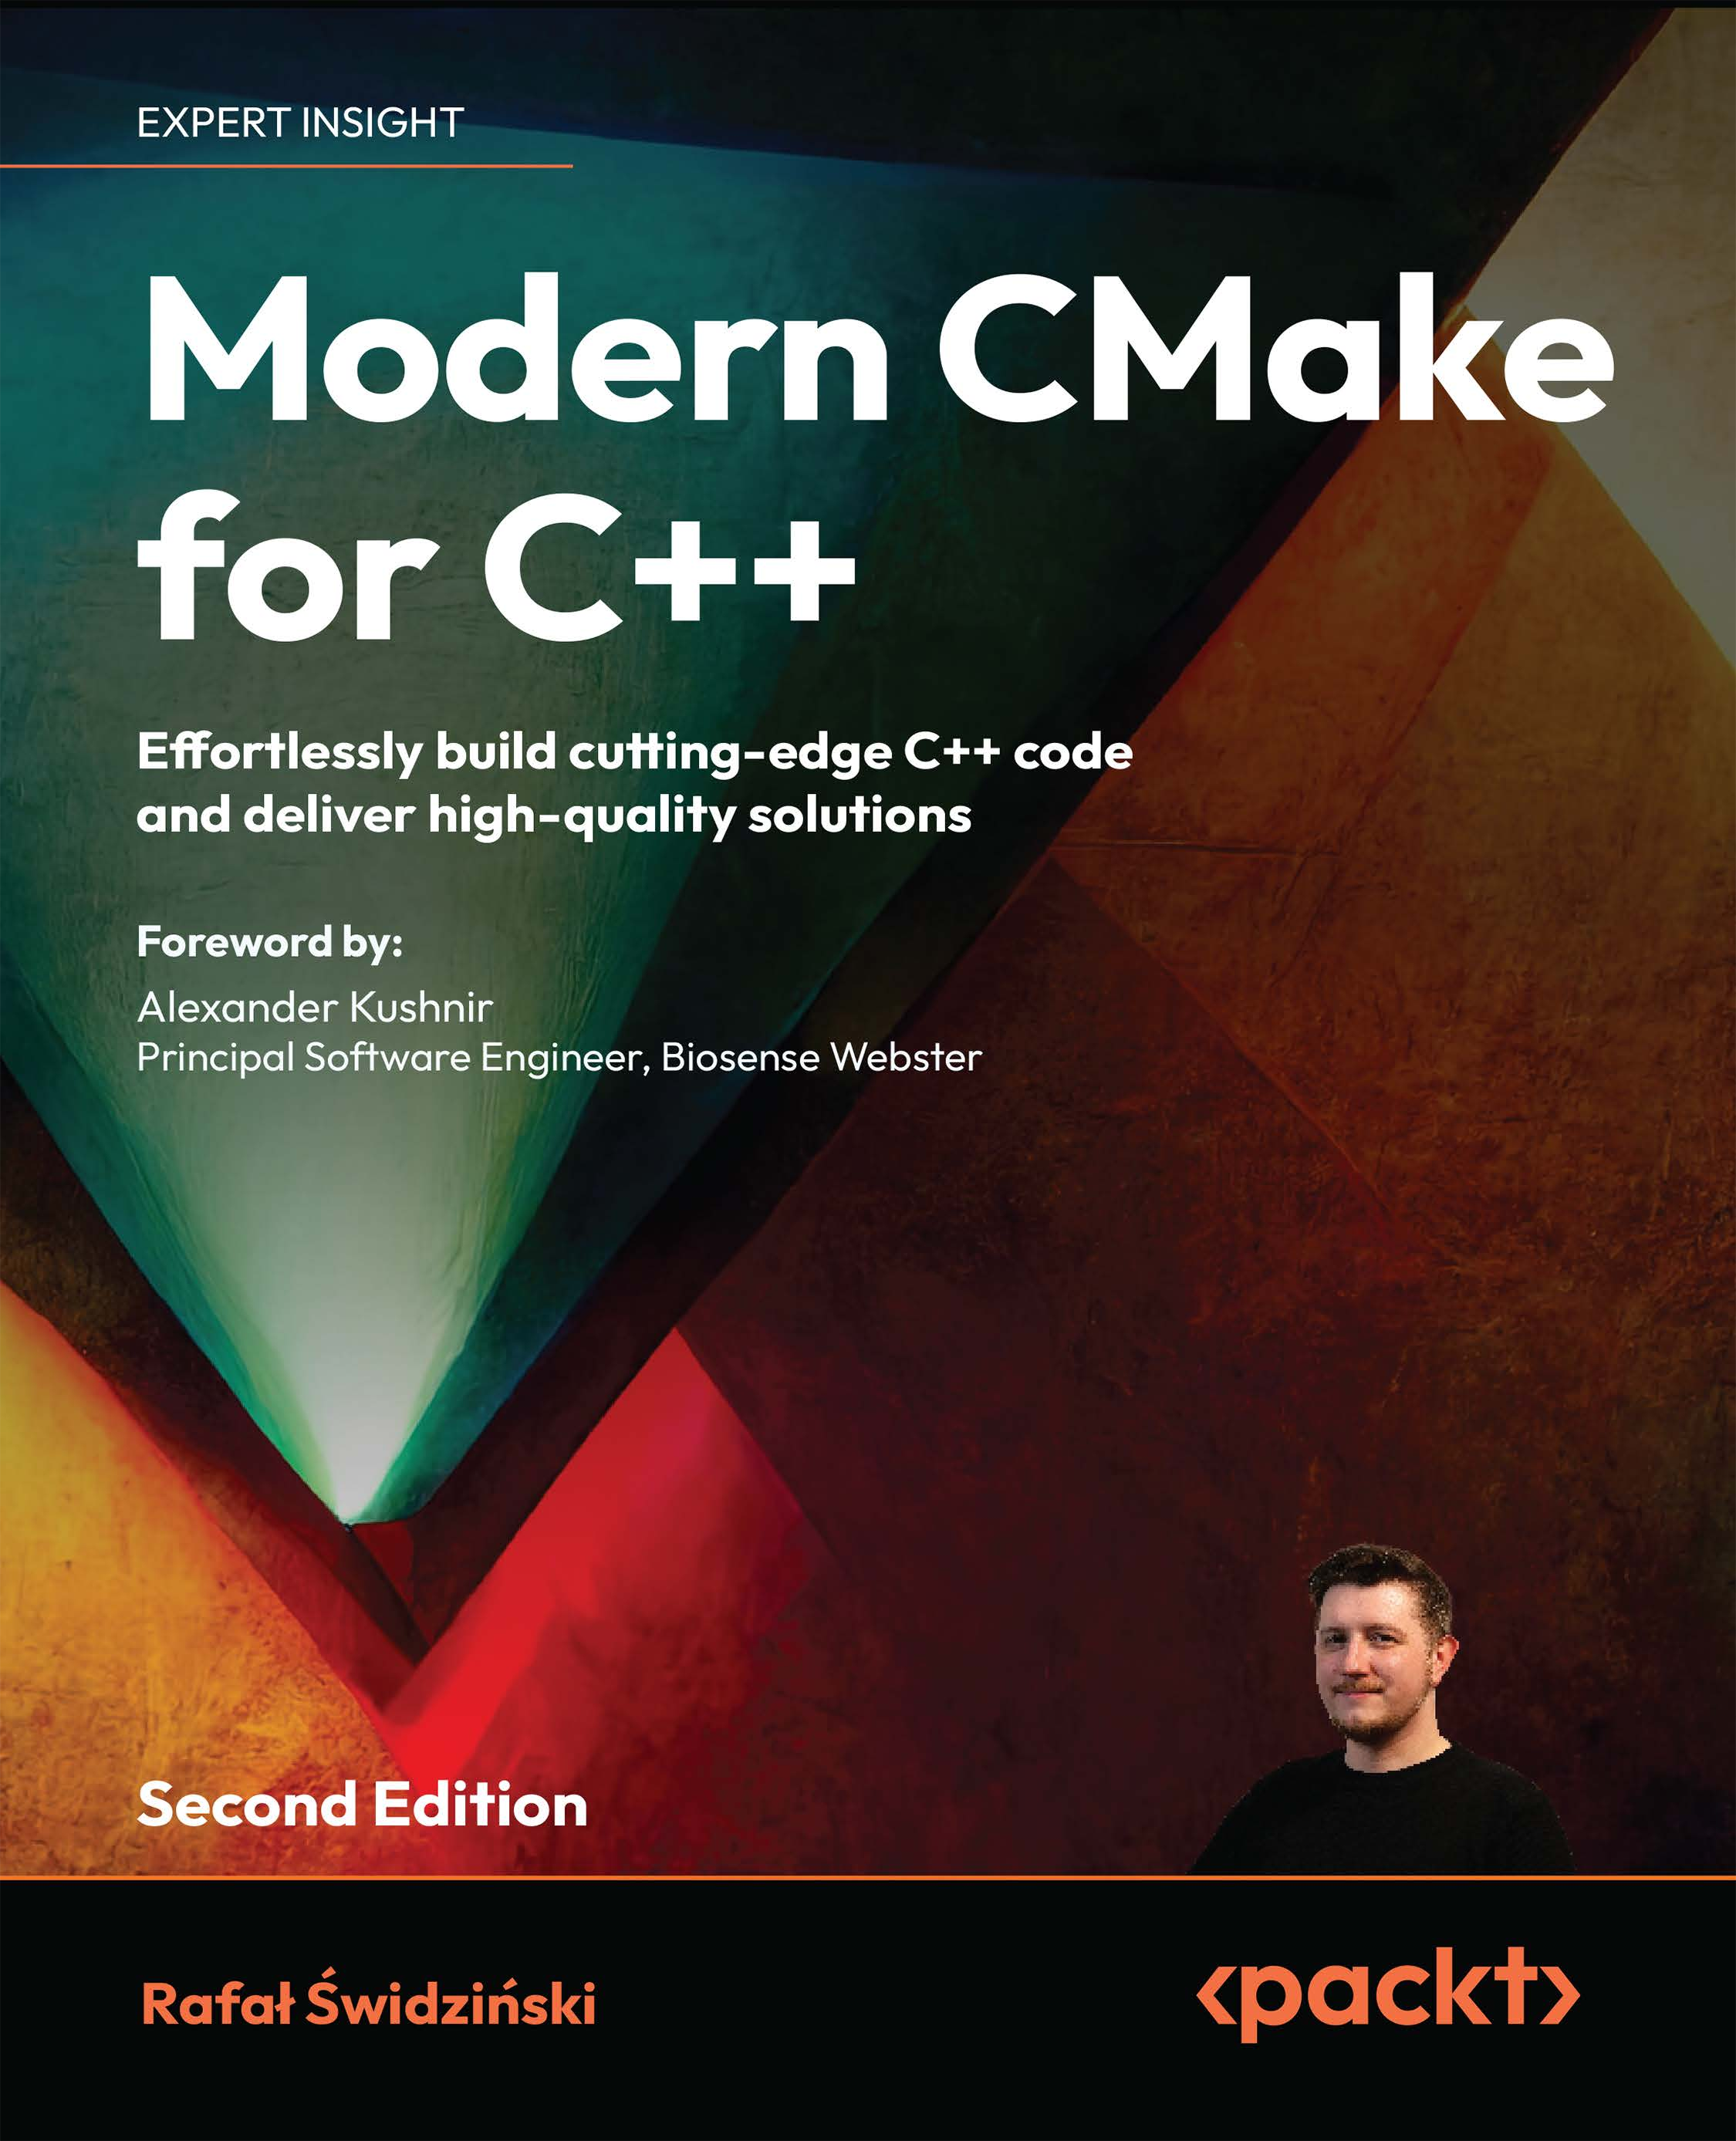
\includegraphics[width=\paperwidth, keepaspectratio=false]{cover.png}};
\end{tikzpicture}
\newpage
\thispagestyle{empty}
\huge
\textbf{Modern CMake for C++ - Second Edition}
\\[9pt]
{\Large 轻松构建前沿C++代码,提供高质量的解决方案}
\\[9pt]
\normalsize
作者: Rafał Świdziński
\\[8pt]
\normalsize
译者:\href{https://github.com/xiaoweiChen/Modern-CMake-for-Cpp-2ed}{陈晓伟}
\\[8pt]
\end{center}

\newpage

\pagestyle{empty}
\tableofcontents
\newpage

\setsecnumdepth{section}

\myPart{}{序}{content/Foreword.tex}
\newpage

\myPart{}{关于作者}{content/Contributors.tex}
\newpage

\myPart{}{关于评审}{content/Reviewers.tex}
\newpage

\myPart{}{前言}{content/Preface.tex}
\newpage

\myChapter{第1章}{使用CMake}{content/chapter1/0.tex}
\mySubsection{1.1.}{示例下载}{content/chapter1/1.tex}
\mySubsection{1.2.}{基本知识}{content/chapter1/2.tex}
\mySubsection{1.3.}{安装CMake}{content/chapter1/3.tex}
\mySubsection{1.4.}{命令行}{content/chapter1/4.tex}
\mySubsection{1.5.}{项目结构}{content/chapter1/5.tex}
\mySubsection{1.6.}{脚本和模块}{content/chapter1/6.tex}
\mySubsection{1.7.}{总结}{content/chapter1/7.tex}
\mySubsection{1.8.}{扩展阅读}{content/chapter1/8.tex}
\newpage

\myChapter{第2章}{CMake语言}{content/chapter2/0.tex}
\mySubsection{2.1.}{示例下载}{content/chapter2/1.tex}
\mySubsection{2.2.}{语法基础}{content/chapter2/2.tex}
\mySubsection{2.3.}{使用变量}{content/chapter2/3.tex}
\mySubsection{2.4.}{使用列表}{content/chapter2/4.tex}
\mySubsection{2.5.}{控制结构}{content/chapter2/5.tex}
\mySubsection{2.6.}{常用命令}{content/chapter2/6.tex}
\mySubsection{2.7.}{总结}{content/chapter2/7.tex}
\mySubsection{2.8.}{扩展阅读}{content/chapter2/8.tex}
\newpage

\myChapter{第3章}{主流的IDE中使用CMake}{content/chapter3/0.tex}
\mySubsection{3.1.}{了解IDE}{content/chapter3/1.tex}
\mySubsection{3.2.}{CLion IDE}{content/chapter3/2.tex}
\mySubsection{3.3.}{Visual Studio Code}{content/chapter3/3.tex}
\mySubsection{3.4.}{Visual Studio IDE}{content/chapter3/4.tex}
\mySubsection{3.5.}{总结}{content/chapter3/5.tex}
\mySubsection{3.6.}{扩展阅读}{content/chapter3/6.tex}
\newpage

\myChapter{第4章}{设置你的第一个CMake项目}{content/chapter4/0.tex}
\mySubsection{4.1.}{示例下载}{content/chapter4/1.tex}
\mySubsection{4.2.}{了解基本的指令和命令}{content/chapter4/2.tex}
\mySubsection{4.3.}{划分项目}{content/chapter4/3.tex}
\mySubsection{4.4.}{项目结构}{content/chapter4/4.tex}
\mySubsection{4.5.}{设置环境范围}{content/chapter4/5.tex}
\mySubsection{4.6.}{配置工具链}{content/chapter4/6.tex}
\mySubsection{4.7.}{禁用源内构建}{content/chapter4/7.tex}
\mySubsection{4.8.}{总结}{content/chapter4/8.tex}
\mySubsection{4.9.}{扩展阅读}{content/chapter4/9.tex}
\newpage

\myChapter{第5章}{与目标一起工作}{content/chapter5/0.tex}
\mySubsection{5.1.}{示例下载}{content/chapter5/1.tex}
\mySubsection{5.2.}{理解目标的概念}{content/chapter5/2.tex}
\mySubsection{5.3.}{编写自定义命令}{content/chapter5/3.tex}
\mySubsection{5.4.}{总结}{content/chapter5/4.tex}
\mySubsection{5.5.}{扩展阅读}{content/chapter5/5.tex}
\newpage

\myChapter{第6章}{使用生成器表达式}{content/chapter6/0.tex}
\mySubsection{6.1.}{示例下载}{content/chapter6/1.tex}
\mySubsection{6.2.}{什么是生成器表达式?}{content/chapter6/2.tex}
\mySubsection{6.3.}{学习通用表达式语法的基本规则}{content/chapter6/3.tex}
\mySubsection{6.4.}{条件扩展}{content/chapter6/4.tex}
\mySubsection{6.5.}{查询和转换}{content/chapter6/5.tex}
\mySubsection{6.6.}{尝试示例}{content/chapter6/6.tex}
\mySubsection{6.7.}{总结}{content/chapter6/7.tex}
\mySubsection{6.8.}{扩展阅读}{content/chapter6/8.tex}
\newpage

\myChapter{第7章}{用CMake编译C++源代码}{content/chapter7/0.tex}
\mySubsection{7.1.}{示例下载}{content/chapter7/1.tex}
\mySubsection{7.2.}{编译的基础}{content/chapter7/2.tex}
\mySubsection{7.3.}{配置预处理器}{content/chapter7/3.tex}
\mySubsection{7.4.}{配置优化器}{content/chapter7/4.tex}
\mySubsection{7.5.}{管理编译过程}{content/chapter7/5.tex}
\mySubsection{7.6.}{总结}{content/chapter7/6.tex}
\mySubsection{7.7.}{扩展阅读}{content/chapter7/7.tex}
\newpage
\end{comment}
\myChapter{第8章}{链接可执行文件和库}{content/chapter8/0.tex}
\mySubsection{8.1.}{示例下载}{content/chapter8/1.tex}
\mySubsection{8.2.}{掌握正确链接的基本知识}{content/chapter8/2.tex}
\mySubsection{8.3.}{构建不同类型的库}{content/chapter8/3.tex}
\mySubsection{8.4.}{解决ODR的问题}{content/chapter8/4.tex}
\mySubsection{8.5.}{连接和未解析符号的顺序}{content/chapter8/5.tex}
\mySubsection{8.6.}{分离main()进行测试}{content/chapter8/6.tex}
\mySubsection{8.7.}{总结}{content/chapter8/7.tex}
\mySubsection{8.8.}{扩展阅读}{content/chapter8/8.tex}
\newpage
\begin{comment}
\myChapter{第9章}{管理依赖关系}{content/chapter9/0.tex}
\mySubsection{9.1.}{示例下载}{content/chapter9/1.tex}
\mySubsection{9.2.}{使用已经安装的依赖项}{content/chapter9/2.tex}
\mySubsection{9.3.}{使用系统中不存在的依赖项}{content/chapter9/3.tex}
\mySubsection{9.4.}{总结}{content/chapter9/4.tex}
\mySubsection{9.5.}{扩展阅读}{content/chapter9/5.tex}
\newpage

\myChapter{第10章}{使用C++20模块}{content/chapter10/0.tex}
\mySubsection{10.1.}{环境准备}{content/chapter10/1.tex}
\mySubsection{10.2.}{C++20模块}{content/chapter10/2.tex}
\mySubsection{10.3.}{使用C++20模块支持编写项目}{content/chapter10/3.tex}
\mySubsection{10.4.}{配置工具链}{content/chapter10/4.tex}
\mySubsection{10.5.}{总结}{content/chapter10/5.tex}
\mySubsection{10.6.}{扩展阅读}{content/chapter10/6.tex}
\newpage

\myChapter{第11章}{测试框架}{content/chapter11/0.tex}
\mySubsection{11.1.}{示例下载}{content/chapter11/1.tex}
\mySubsection{11.2.}{为什么要自动化测试?}{content/chapter11/2.tex}
\mySubsection{11.3.}{使用CTest在CMake中标准化测试}{content/chapter11/3.tex}
\mySubsection{11.4.}{为CTest创建最基本的单元测试}{content/chapter11/4.tex}
\mySubsection{11.5.}{为测试构建项目}{content/chapter11/5.tex}
\mySubsection{11.6.}{单元测试框架}{content/chapter11/6.tex}
\mySubsection{11.7.}{生成测试覆盖率报告}{content/chapter11/7.tex}
\mySubsection{11.8.}{总结}{content/chapter11/8.tex}
\mySubsection{11.9.}{扩展阅读}{content/chapter11/9.tex}
\newpage

\myChapter{第12章}{程序分析工具}{content/chapter12/0.tex}
\mySubsection{12.1.}{示例下载}{content/chapter12/1.tex}
\mySubsection{12.2.}{执行格式化}{content/chapter12/2.tex}
\mySubsection{12.3.}{使用静态检查器}{content/chapter12/3.tex}
\mySubsection{12.4.}{动态分析与Valgrind}{content/chapter12/4.tex}
\mySubsection{12.5.}{总结}{content/chapter12/5.tex}
\mySubsection{12.6.}{扩展阅读}{content/chapter12/6.tex}
\newpage

\myChapter{第13章}{程序分析工具}{content/chapter13/0.tex}
\mySubsection{13.1.}{示例下载}{content/chapter13/1.tex}
\mySubsection{13.2.}{添加Doxygen到项目中}{content/chapter13/2.tex}
\mySubsection{13.3.}{生成具有现代外观的文档}{content/chapter13/3.tex}
\mySubsection{13.4.}{使用自定义HTML增强输出}{content/chapter13/4.tex}
\mySubsection{13.5.}{总结}{content/chapter13/5.tex}
\mySubsection{13.6.}{扩展阅读}{content/chapter13/6.tex}
\newpage

\myChapter{第14章}{安装与打包}{content/chapter14/0.tex}
\mySubsection{14.1.}{示例下载}{content/chapter14/1.tex}
\mySubsection{14.2.}{导出而不安装}{content/chapter14/2.tex}
\mySubsection{14.3.}{在系统上安装项目}{content/chapter14/3.tex}
\mySubsection{14.4.}{创建可重用的包}{content/chapter14/4.tex}
\mySubsection{14.5.}{定义组件}{content/chapter14/5.tex}
\mySubsection{14.6.}{使用CPack}{content/chapter14/6.tex}
\mySubsection{14.7.}{总结}{content/chapter14/7.tex}
\mySubsection{14.8.}{扩展阅读}{content/chapter14/8.tex}
\newpage

\myChapter{第15章}{创建你的专业项目}{content/chapter15/0.tex}
\mySubsection{15.1.}{示例下载}{content/chapter15/1.tex}
\mySubsection{15.2.}{计划工作}{content/chapter15/2.tex}
\mySubsection{15.3.}{项目布局}{content/chapter15/3.tex}
\mySubsection{15.4.}{构建和管理依赖关系}{content/chapter15/4.tex}
\mySubsection{15.5.}{测试和程序分析}{content/chapter15/5.tex}
\mySubsection{15.6.}{安装与打包}{content/chapter15/6.tex}
\mySubsection{15.7.}{提供文档}{content/chapter15/7.tex}
\mySubsection{15.8.}{总结}{content/chapter15/8.tex}
\mySubsection{15.9.}{扩展阅读}{content/chapter15/9.tex}
\newpage

\myChapter{第16章}{编写CMake预设}{content/chapter16/0.tex}
\mySubsection{16.1.}{示例下载}{content/chapter16/1.tex}
\mySubsection{16.2.}{使用项目中定义的预设}{content/chapter16/2.tex}
\mySubsection{16.3.}{编写预设文件}{content/chapter16/3.tex}
\mySubsection{16.4.}{特定阶段的预设}{content/chapter16/4.tex}
\mySubsection{16.5.}{定义工作流预设}{content/chapter16/5.tex}
\mySubsection{16.6.}{添加条件和宏}{content/chapter16/6.tex}
\mySubsection{16.7.}{总结}{content/chapter16/7.tex}
\mySubsection{16.8.}{扩展阅读}{content/chapter16/8.tex}
\newpage

\myChapter{附录}{}{content/chapter17/0.tex}
\mySubsection{17.1.}{其他命令}{content/chapter17/1.tex}
\mySubsection{17.2.}{string()}{content/chapter17/2.tex}
\mySubsection{17.3.}{list()}{content/chapter17/3.tex}
\mySubsection{17.4.}{file()}{content/chapter17/4.tex}
\mySubsection{17.5.}{math()}{content/chapter17/5.tex}
\newpage


\end{comment}